\documentclass[conference]{IEEEtran}

\IEEEoverridecommandlockouts
% Add the compsoc option for Computer Society conferences.
%
% If IEEEtran.cls has not been installed into the LaTeX system files,
% manually specify the path to it like:
% \documentclass[conference]{../sty/IEEEtran}


\usepackage{listings}
\usepackage{url}
\usepackage{graphicx}
\usepackage{numprint}
\usepackage{array,multirow}
\usepackage{multicol}
\usepackage{amssymb}
\usepackage{tikz}
\usepackage[autostyle]{csquotes}



\newtheorem{rem}{Remark}
\newtheorem{example}{Example}
% Some very useful LaTeX packages include:
% (uncomment the ones you want to load)


% *** MISC UTILITY PACKAGES ***
%
%\usepackage{ifpdf}
% Heiko Oberdiek's ifpdf.sty is very useful if you need conditional
% compilation based on whether the output is pdf or dvi.
% usage:
% \ifpdf
%   % pdf code
% \else
%   % dvi code
% \fi
% The latest version of ifpdf.sty can be obtained from:
% http://www.ctan.org/tex-archive/macros/latex/contrib/oberdiek/
% Also, note that IEEEtran.cls V1.7 and later provides a builtin
% \ifCLASSINFOpdf conditional that works the same way.
% When switching from latex to pdflatex and vice-versa, the compiler may
% have to be run twice to clear warning/error messages.






% *** CITATION PACKAGES ***
%
%\usepackage{cite}
% cite.sty was written by Donald Arseneau
% V1.6 and later of IEEEtran pre-defines the format of the cite.sty package
% \cite{} output to follow that of IEEE. Loading the cite package will
% result in citation numbers being automatically sorted and properly
% "compressed/ranged". e.g., [1], [9], [2], [7], [5], [6] without using
% cite.sty will become [1], [2], [5]--[7], [9] using cite.sty. cite.sty's
% \cite will automatically add leading space, if needed. Use cite.sty's
% noadjust option (cite.sty V3.8 and later) if you want to turn this off.
% cite.sty is already installed on most LaTeX systems. Be sure and use
% version 4.0 (2003-05-27) and later if using hyperref.sty. cite.sty does
% not currently provide for hyperlinked citations.
% The latest version can be obtained at:
% http://www.ctan.org/tex-archive/macros/latex/contrib/cite/
% The documentation is contained in the cite.sty file itself.






% *** GRAPHICS RELATED PACKAGES ***
%
\ifCLASSINFOpdf
  % \usepackage[pdftex]{graphicx}
  % declare the path(s) where your graphic files are
  % \graphicspath{{../pdf/}{../jpeg/}}
  % and their extensions so you won't have to specify these with
  % every instance of \includegraphics
  % \DeclareGraphicsExtensions{.pdf,.jpeg,.png}
\else
  % or other class option (dvipsone, dvipdf, if not using dvips). graphicx
  % will default to the driver specified in the system graphics.cfg if no
  % driver is specified.
  % \usepackage[dvips]{graphicx}
  % declare the path(s) where your graphic files are
  % \graphicspath{{../eps/}}
  % and their extensions so you won't have to specify these with
  % every instance of \includegraphics
  % \DeclareGraphicsExtensions{.eps}
\fi
% graphicx was written by David Carlisle and Sebastian Rahtz. It is
% required if you want graphics, photos, etc. graphicx.sty is already
% installed on most LaTeX systems. The latest version and documentation can
% be obtained at:
% http://www.ctan.org/tex-archive/macros/latex/required/graphics/
% Another good source of documentation is "Using Imported Graphics in
% LaTeX2e" by Keith Reckdahl which can be found as epslatex.ps or
% epslatex.pdf at: http://www.ctan.org/tex-archive/info/
%
% latex, and pdflatex in dvi mode, support graphics in encapsulated
% postscript (.eps) format. pdflatex in pdf mode supports graphics
% in .pdf, .jpeg, .png and .mps (metapost) formats. Users should ensure
% that all non-photo figures use a vector format (.eps, .pdf, .mps) and
% not a bitmapped formats (.jpeg, .png). IEEE frowns on bitmapped formats
% which can result in "jaggedy"/blurry rendering of lines and letters as
% well as large increases in file sizes.
%
% You can find documentation about the pdfTeX application at:
% http://www.tug.org/applications/pdftex





% *** MATH PACKAGES ***
%
%\usepackage[cmex10]{amsmath}
% A popular package from the American Mathematical Society that provides
% many useful and powerful commands for dealing with mathematics. If using
% it, be sure to load this package with the cmex10 option to ensure that
% only type 1 fonts will utilized at all point sizes. Without this option,
% it is possible that some math symbols, particularly those within
% footnotes, will be rendered in bitmap form which will result in a
% document that can not be IEEE Xplore compliant!
%
% Also, note that the amsmath package sets \interdisplaylinepenalty to 10000
% thus preventing page breaks from occurring within multiline equations. Use:
%\interdisplaylinepenalty=2500
% after loading amsmath to restore such page breaks as IEEEtran.cls normally
% does. amsmath.sty is already installed on most LaTeX systems. The latest
% version and documentation can be obtained at:
% http://www.ctan.org/tex-archive/macros/latex/required/amslatex/math/





% *** SPECIALIZED LIST PACKAGES ***
%
%\usepackage{algorithmic}
% algorithmic.sty was written by Peter Williams and Rogerio Brito.
% This package provides an algorithmic environment fo describing algorithms.
% You can use the algorithmic environment in-text or within a figure
% environment to provide for a floating algorithm. Do NOT use the algorithm
% floating environment provided by algorithm.sty (by the same authors) or
% algorithm2e.sty (by Christophe Fiorio) as IEEE does not use dedicated
% algorithm float types and packages that provide these will not provide
% correct IEEE style captions. The latest version and documentation of
% algorithmic.sty can be obtained at:
% http://www.ctan.org/tex-archive/macros/latex/contrib/algorithms/
% There is also a support site at:
% http://algorithms.berlios.de/index.html
% Also of interest may be the (relatively newer and more customizable)
% algorithmicx.sty package by Szasz Janos:
% http://www.ctan.org/tex-archive/macros/latex/contrib/algorithmicx/




% *** ALIGNMENT PACKAGES ***
%
%\usepackage{array}
% Frank Mittelbach's and David Carlisle's array.sty patches and improves
% the standard LaTeX2e array and tabular environments to provide better
% appearance and additional user controls. As the default LaTeX2e table
% generation code is lacking to the point of almost being broken with
% respect to the quality of the end results, all users are strongly
% advised to use an enhanced (at the very least that provided by array.sty)
% set of table tools. array.sty is already installed on most systems. The
% latest version and documentation can be obtained at:
% http://www.ctan.org/tex-archive/macros/latex/required/tools/


%\usepackage{mdwmath}
%\usepackage{mdwtab}
% Also highly recommended is Mark Wooding's extremely powerful MDW tools,
% especially mdwmath.sty and mdwtab.sty which are used to format equations
% and tables, respectively. The MDWtools set is already installed on most
% LaTeX systems. The lastest version and documentation is available at:
% http://www.ctan.org/tex-archive/macros/latex/contrib/mdwtools/


% IEEEtran contains the IEEEeqnarray family of commands that can be used to
% generate multiline equations as well as matrices, tables, etc., of high
% quality.


%\usepackage{eqparbox}
% Also of notable interest is Scott Pakin's eqparbox package for creating
% (automatically sized) equal width boxes - aka "natural width parboxes".
% Available at:
% http://www.ctan.org/tex-archive/macros/latex/contrib/eqparbox/





% *** SUBFIGURE PACKAGES ***
%\usepackage[tight,footnotesize]{subfigure}
% subfigure.sty was written by Steven Douglas Cochran. This package makes it
% easy to put subfigures in your figures. e.g., "Figure 1a and 1b". For IEEE
% work, it is a good idea to load it with the tight package option to reduce
% the amount of white space around the subfigures. subfigure.sty is already
% installed on most LaTeX systems. The latest version and documentation can
% be obtained at:
% http://www.ctan.org/tex-archive/obsolete/macros/latex/contrib/subfigure/
% subfigure.sty has been superceeded by subfig.sty.



%\usepackage[caption=false]{caption}
%\usepackage[font=footnotesize]{subfig}
% subfig.sty, also written by Steven Douglas Cochran, is the modern
% replacement for subfigure.sty. However, subfig.sty requires and
% automatically loads Axel Sommerfeldt's caption.sty which will override
% IEEEtran.cls handling of captions and this will result in nonIEEE style
% figure/table captions. To prevent this problem, be sure and preload
% caption.sty with its "caption=false" package option. This is will preserve
% IEEEtran.cls handing of captions. Version 1.3 (2005/06/28) and later
% (recommended due to many improvements over 1.2) of subfig.sty supports
% the caption=false option directly:
%\usepackage[caption=false,font=footnotesize]{subfig}
%
% The latest version and documentation can be obtained at:
% http://www.ctan.org/tex-archive/macros/latex/contrib/subfig/
% The latest version and documentation of caption.sty can be obtained at:
% http://www.ctan.org/tex-archive/macros/latex/contrib/caption/




% *** FLOAT PACKAGES ***
%
%\usepackage{fixltx2e}
% fixltx2e, the successor to the earlier fix2col.sty, was written by
% Frank Mittelbach and David Carlisle. This package corrects a few problems
% in the LaTeX2e kernel, the most notable of which is that in current
% LaTeX2e releases, the ordering of single and double column floats is not
% guaranteed to be preserved. Thus, an unpatched LaTeX2e can allow a
% single column figure to be placed prior to an earlier double column
% figure. The latest version and documentation can be found at:
% http://www.ctan.org/tex-archive/macros/latex/base/



%\usepackage{stfloats}
% stfloats.sty was written by Sigitas Tolusis. This package gives LaTeX2e
% the ability to do double column floats at the bottom of the page as well
% as the top. (e.g., "\begin{figure*}[!b]" is not normally possible in
% LaTeX2e). It also provides a command:
%\fnbelowfloat
% to enable the placement of footnotes below bottom floats (the standard
% LaTeX2e kernel puts them above bottom floats). This is an invasive package
% which rewrites many portions of the LaTeX2e float routines. It may not work
% with other packages that modify the LaTeX2e float routines. The latest
% version and documentation can be obtained at:
% http://www.ctan.org/tex-archive/macros/latex/contrib/sttools/
% Documentation is contained in the stfloats.sty comments as well as in the
% presfull.pdf file. Do not use the stfloats baselinefloat ability as IEEE
% does not allow \baselineskip to stretch. Authors submitting work to the
% IEEE should note that IEEE rarely uses double column equations and
% that authors should try to avoid such use. Do not be tempted to use the
% cuted.sty or midfloat.sty packages (also by Sigitas Tolusis) as IEEE does
% not format its papers in such ways.





% *** PDF, URL AND HYPERLINK PACKAGES ***
%
%\usepackage{url}
% url.sty was written by Donald Arseneau. It provides better support for
% handling and breaking URLs. url.sty is already installed on most LaTeX
% systems. The latest version can be obtained at:
% http://www.ctan.org/tex-archive/macros/latex/contrib/misc/
% Read the url.sty source comments for usage information. Basically,
% \url{my_url_here}.


% *** Do not adjust lengths that control margins, column widths, etc. ***
% *** Do not use packages that alter fonts (such as pslatex).         ***
% There should be no need to do such things with IEEEtran.cls V1.6 and later.
% (Unless specifically asked to do so by the journal or conference you plan
% to submit to, of course. )


% correct bad hyphenation here
\hyphenation{op-tical net-works semi-conduc-tor}

\def \ICSTW {2017 IEEE Eighth International Conference on Software Testing, Verification and Validation Workshops (ICSTW)}
\def \TAICPART {10th Testing: Academic and Industrial Conference - Practice and Research Techniques (TAIC PART)}
\def \SECTEST {6th International Workshop on Security Testing (SECTEST 2015)}
\def \MUTATION {10th International Workshop on Mutation Analysis (Mutation 2015)}
\def \IWCT {Submitted for publication to 6th International Workshop on Combinatorial Testing (IWCT 2017)}
\def \INSTA {2nd International Workshop on Software Test Architecture (InSTA 2015)}
\def \AMOST {12th Workshop on Advances in Model Based Testing (A-MOST 2015)}
\def \ASQT {13th User Symposium on Software Quality, Test and Innovation (ASQT 2015)}

\def \UScopyright {U.S. Government work not protected by U.S. copyright}
\def \UKcopyright {978-1-4799-1885-0/15/\$31.00 \copyright 2015 Crown}
\def \EUcopyright {978-1-4799-1885-0/15/\$31.00 \copyright 2015 European Union}
\def \IEEEcopyright {978-1-4799-1885-0/15/\$31.00 \copyright 2015 IEEE}

\newcommand{\copyrights}[2]{%
\renewcommand{\thefootnote}{}%
\footnotetext{\ICSTW \\ #1 \\ #2}
\renewcommand{\thefootnote}{\arabic{footnote}}%
}

\usepackage{color}
\newcommand{\todo}[1]{}
\renewcommand{\todo}[1]{{\color{red} TODO: {#1}}}

\usepackage{listings,xcolor}

\begin{document}


\title{An Industrial Study on Applications of Combinatorial Testing in Modern Web Development}


\author{\IEEEauthorblockN{Murat Ozcan}
\IEEEauthorblockA{Siemens Building Technologies CPS Software Hub\\
Chicago, USA\\
murat.ozcan@siemens.com}
}

\maketitle


\begin{abstract}
The purpose of this study is to describe the new paradigms in front-end web application testing and how combinatorial testing (CT) fits in this modern development environment to create cost effective, highly fault-detecting automated tests.
The system under test (SUT) is a cloud based application for monitoring and controlling building operations from Siemens Building Technologies, currently under development.

Three examples for the applications of combinatorial testing in the front-end are analyzed,
incorporating the CT model into automation using Protractor test framework's end-to-end (e2e) UI tests in behavioral driven development (BDD) style. 
The manner in which the CT model translates automation code is studied.
A scenario where a sequence of actions are incorporated into a CT model is illustrated;
with a focus on verification of these sequences, compositions of the actions and streamlining the expected assertions per the test oracle.

\end{abstract}

\begin{IEEEkeywords}
Cloud, combinatorial testing, sequence, test automation, Docker, Angular, Protractor
\end{IEEEkeywords}

\section{Introduction}

In this paper we will showcase how CT fits in the front-end test automation in a continuous integration (CI) environment.
Examples will include modeling of the input parameter model (IPM) and how the model translates to test code.
One example will include a scenario where a sequence of actions will be incorporated into a CT model, a problem that has been addressed in a variety of ways in previous works.

Due to space constraints, this study will focus on black box test automation of the front-end.
The CI environment will be described, however CT applications in the CI pipeline and testing at different levels of the architecture are not the focus of the paper, they are planned for a future effort.

\section{Related Work}

	Existing studies have focused on integrating covering arrays and sequence testing \cite{kuhn2012combinatorial}, \cite{farchi2014combinatorial}, \cite{brain2012event}.
	In comparison, the method of modeling sequenced parameter groups applied in this paper is to solve a simpler problem:
	to incorporate testing three test actions in their varying sequences, without increasing the number of tests achieved using a covering array which does not factor-in sequences of these three test actions.
	Constraints are the driving factor behind the logic. Implementation borrows ideas from a combination of the modeling patterns found in the previous work on sequences as well as other common patterns in CT \cite{segall2012common}, which include: 
	\begin{itemize}
		\item \textit{Optional and conditionally-excluded values:} the use of N/A value for parameters that are not a part of the parameter group in the current sequence.
		\item	\textit{Multi-selection \& Order and padding:} a variation of these ideas was used for sequence control parameters.
		\item \textit{Equivalence partitioning \& Boundary value analysis:} used in input parameter modeling.
	\end{itemize}

\section{The System Under Test}
	\subsection{Description of the Architecture}
	
	The SUT under development is a cloud application utilizing microservices, that enables the users to connect to their buildings though a browser interface, monitor and operate the buildings remotely.
	The front-end of the SUT is an Angular framework in TypeScript.
	The back-end is an ExpressJS application on top of the NodeJS platform. 
	Further backend components serve the purpose of exposing Siemens or third-party edge-devices to the cloud.

	\subsection{Description of the CI Environment }
	
	The team uses GitLab for CI.
	When any code is submitted, the application is built in a docker container, unit testing and linting are done, the container containing the application is deployed and run in a cloud-hosted container and finally automated UI tests are executed targeting this deployment.
	If testing passes, the code can get merged to the master branch. 
	This automated testing process ensures that after any code commit, the application is fully regression tested and quality is ensured. 

\subsection{Description of the Test Code}

	\subsubsection{Test data}
	The test data is stored in JavaScript Object Notation (JSON) files. 
	This allows parameterization of test inputs, input-driven tests, as well as ease of maintenance as the test configurations or the UI changes.
	It was found that another perk of using JSON is being able to convert test suites generated with CT tools from csv format to JSON format.

	\subsubsection{Test Specifications}

	The team uses Protractor test framework, which is the default e2e test framework for Angular applications.
	The test specifications are stored in Protractor spec files written in TypeScript. 

\section{Test Methodology}

	In the following sections test designs using CT techniques will be described. 
	For all CT suite generation CTWedge \cite{gargantini2018migrating} was used and for coverage measuring CAMetrics \cite{leithner2018cametrics} was used.
	In all IPMs, a partial script is shown due to space constraints. They can be provided upon request.
	The CT test design and test automation workflow in all subsections is as such:
	\begin{enumerate}
		\item CT modeling of the IPM as in CTWedge script snippet.
		\item Generation of test suite in csv, conversion to JSON.
		\item Based on the test suite, writing the automated test code.
	\end{enumerate}
	
	\subsection{Input driven testing of hardware} \label{Input driven testing of hardware}
	
	The IPM for the hardware test configuration is agnostic to device types and building control points.
	This is achieved through parameters and values in JSON format.
	The following code snippet shows how the input parameters and their values are represented in JSON. 
	For example, a binary-output point which may control a digital light or a fan may be referred to as \textit{FanCmd} (Fan Command) or \textit{LDO} (Logical Digital Output).
  Through parameterization this complexity is abstracted. The test code only uses the parameters and the values of the parameters are easily manipulated depending on UI changes and or test configurations.
		
	\lstset{
    string=[s]{"}{"},
    stringstyle=\color{blue},
    comment=[l]{:},
		commentstyle=\color{black},
		tabsize = 1, %% Sets tab space width.
		showstringspaces = false, %% Prevents space marking in strings, string is defined as the text that is generally printed directly to the console.
		%numbers = left, %% Displays line numbers on the left.
		keywordstyle = \color{blue}, %% Sets  keyword color.
		stringstyle = \color{red}, %% Sets  string color.
		rulecolor = \color{black}, %% Sets frame color to avoid being affected by text color.
		basicstyle = \footnotesize  \ttfamily , %% Sets listing font and size.
		breaklines = true, %% Enables line breaking.
		numberstyle = \tiny,
	}
	\begin{lstlisting}
		"SubSystemType": {
			"SystemOne": "DXR-VAV",
			"DesigoClassic": "DesigoClassic-ASG03",
			"ApogeeBACnetFLN": "PTEC-Heat_Pump"
		},
		"PointType_SystemOne": {
			"AnalogValue": "ECO CLG STPT",
			"BinaryOutput": "FAN 1 SPD 2" ....
		}
	\end{lstlisting}

	In the CTWedge script snippet, it can be observed that the parameters \emph{subsystemType} and \emph{pointType} map directly from JSON data.
	On the other hand, parameters such as \emph{commandType} and \emph{commandToPointValue} represent abstracted test actions.
	All possible test actions are defined in the parameters and later, depending on the type of point, are restricted through constraints.
	Verbal description of constraints are included as comments in the CT model, easing readability.

	\lstset{
    string=[s]{"}{"},
    stringstyle=\color{blue},
    comment=[l]{:},
		commentstyle=\color{black},
		tabsize = 1, %% Sets tab space width.W
		showstringspaces = false, %% Prevents space marking in strings, string is defined as the text that is generally printed directly to the console.
		%numbers = left, %% Displays line numbers on the left.
		keywordstyle = \color{blue}, %% Sets  keyword color.
		stringstyle = \color{red}, %% Sets  string color.
		rulecolor = \color{black}, %% Sets frame color to avoid being affected by text color.
		basicstyle = \footnotesize  \ttfamily , %% Sets listing font and size.
		breaklines = true, %% Enables line breaking.
		numberstyle = \tiny,
	}
	\begin{lstlisting}
	Model Commanding
	Parameters:
		subsytemType : {ApogeeBACnet, ApogeeBACnetFLN, 3rdPartyBACnet, Modbus, DesigoClassic, SystemOne, SystemOneAX100}
		pointType:  {BO, MO, AO, BV, MV, AV, BI, AI, HoldingReg1, HoldingReg2}  
		commandType: {slider, buttons_plusMinus, textBox, buttonsOnOff, buttons3stages, NA}
		commandToPointValue: { readOnly, cancel, anyValue, higherByOne, lowerByOne, lowBoundary, highBoundary, lowBoundaryBeyond, highBoundaryBeyond}			
	 Constraints:
	 // if pointType is BO or BV, you can only command it +1, -1, cancel, command type is fixed to OnOff and it's not readOnly
	 # (pointType = BO) || (pointType = BV) => ((commandToPointValue = higherByOne) || (commandToPointValue = lowerByOne) || (commandToPointValue = cancel)) && (commandType = buttonsOnOff) && (commandToPointValue != readOnly) # 
	 // if pointType is MO or MV, you can only command it +1 (and another), -1 (and another), cancel, command type is fixed to buttons3stages and it's not readOnly
	 # (pointType = MO) || (pointType = MV) => ((commandToPointValue = higherByOne) || (commandToPointValue = lowerByOne) || (commandToPointValue = cancel)) && (commandType = buttons3stages) && (commandToPointValue != readOnly) # 
	\end{lstlisting}

	Binary points and Multi-state points have two or more states, followed by confirm or cancel commands. 
	Certain points such as inputs may be \textit{readOnly} and do not have a \textit{commandType}. Such points have a \textit{N/A} value for \textit{commandType}, and the parameter is \textit{negated} through its use; a CT technique described in \cite{segall2012common}.	

	Compared to binary and multistate points, analog points are more complex and have a variety of command options.
	They can be commanded via slider, text box, incremented or decremented. 
	They are prime candidates for boundary value analysis and equivalence partitioning in CT \cite{segall2012common}.

	\begin{figure}[!t]
		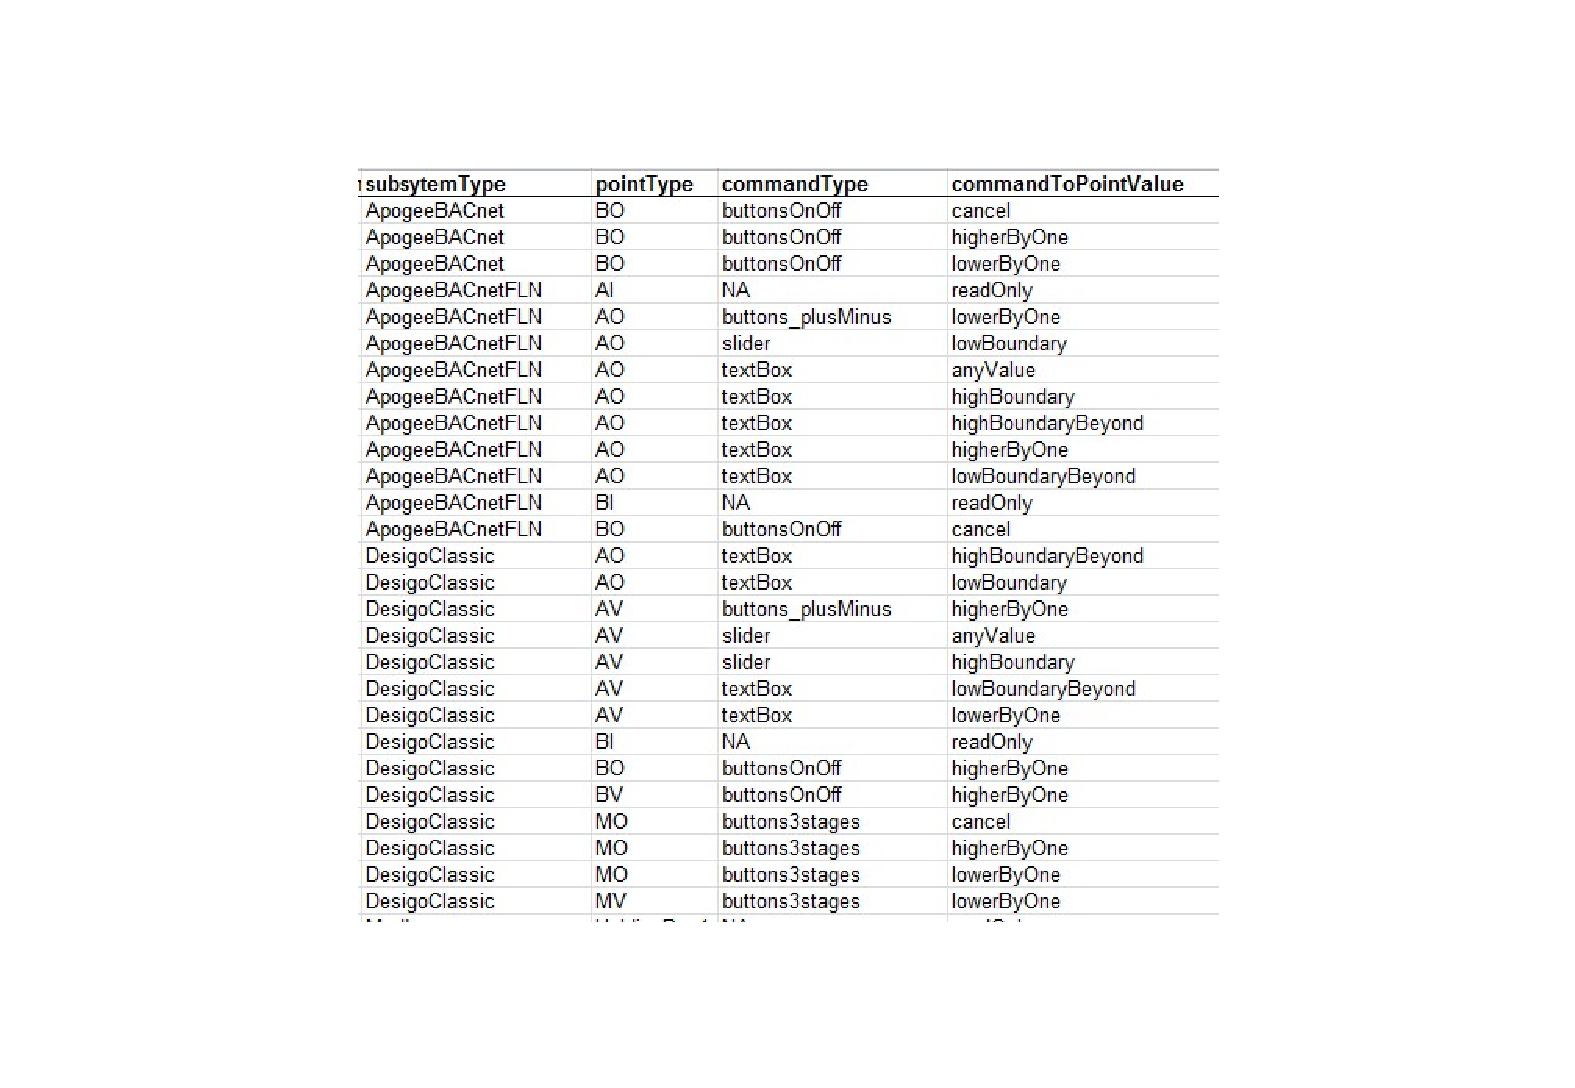
\includegraphics[width=0.45\textwidth,]{csvOutputCommanding.pdf}
		\caption{Partial input driven commanding test suite}
		\label{fig:csvOutputCommanding}
	\end{figure}

	It is our opinion that the test suite in Figure~\ref{fig:csvOutputCommanding} and test code snippet will solidify the understanding of the application of constraints for analog points.
	For ease of readability and confidentiality, test actions and assertions are handled under the functions in the code snippet. 

	\lstset{
    string=[s]{"}{"},
    stringstyle=\color{blue},
    comment=[l]{:},
		commentstyle=\color{black},
		tabsize = 1, %% Sets tab space width.
		showstringspaces = false, %% Prevents space marking in strings, string is defined as the text that is generally printed directly to the console.
		%numbers = left, %% Displays line numbers on the left.
		keywordstyle = \color{blue}, %% Sets  keyword color.
		stringstyle = \color{red}, %% Sets  string color.
		rulecolor = \color{black}, %% Sets frame color to avoid being affected by text color.
		basicstyle = \footnotesize  \ttfamily , %% Sets listing font and size.
		breaklines = true, %% Enables line breaking.
		numberstyle = \tiny,
	}
	\begin{lstlisting}
	describe('Testing commanding', () => {
		it('analog point, slider high bound.', () => {
			pointCommand.slider.highBoundary(); });
		it('analog point, (+) button', () => {
			pointCommand.button.incrementValue();	}); 
		});
	\end{lstlisting}

	\subsection{Filtering Points by Tag Combinations }

	In the building technologies domain, a point is any object used to control the building; i.e. a light switch can be a digital point, a thermostat can be an analog point.
	In the SUT, tag filtering functionality is used to filter points in the system, by the devices the points are in.
	There are 13 possible tags, up to 5 tags can be chosen, tag choices cannot repeat, the final tag has only one tag choice, and there can be less than 5 tags for certain tag combinations if so is the nature of the points in the system.
	The following CTWedge script samples the IPM of the functionality.
	The constraint logic is that no tag can repeat, with 4 constraints for each tag.

	\lstset{
    string=[s]{"}{"},
    stringstyle=\color{blue},
    comment=[l]{:},
		commentstyle=\color{black},
		tabsize = 1, %% Sets tab space width.
		showstringspaces = false, %% Prevents space marking in strings, string is defined as the text that is generally printed directly to the console.
		%numbers = left, %% Displays line numbers on the left.
		keywordstyle = \color{blue}, %% Sets  keyword color.
		stringstyle = \color{red}, %% Sets  string color.
		rulecolor = \color{black}, %% Sets frame color to avoid being affected by text color.
		basicstyle = \footnotesize  \ttfamily , %% Sets listing font and size.
		breaklines = true, %% Enables line breaking.
		numberstyle = \tiny,
	}
	\begin{lstlisting}
		Model tags
		Parameters:
			tag1 : {cmd, writable, sensor, temp, cooling..}
			tag2 : {cmd, writable, sensor, temp, cooling..}
			tag3 : {cmd, writable, sensor, temp, cooling..}
			tag4 : {cmd, writable, sensor, temp, cooling..}
	 Constraints:
		// can't duplicate tags!
		# tag1=cmd => tag2!=cmd && tag3!=cmd ..
		# tag2=cmd => tag1!=cmd && tag3!=cmd ..
		# tag3=cmd => tag2!=cmd && tag1!=cmd ..
		# tag4=cmd => tag2!=cmd && tag3!=cmd ..#
	\end{lstlisting}

	\begin{figure}[!t]
		\centering
		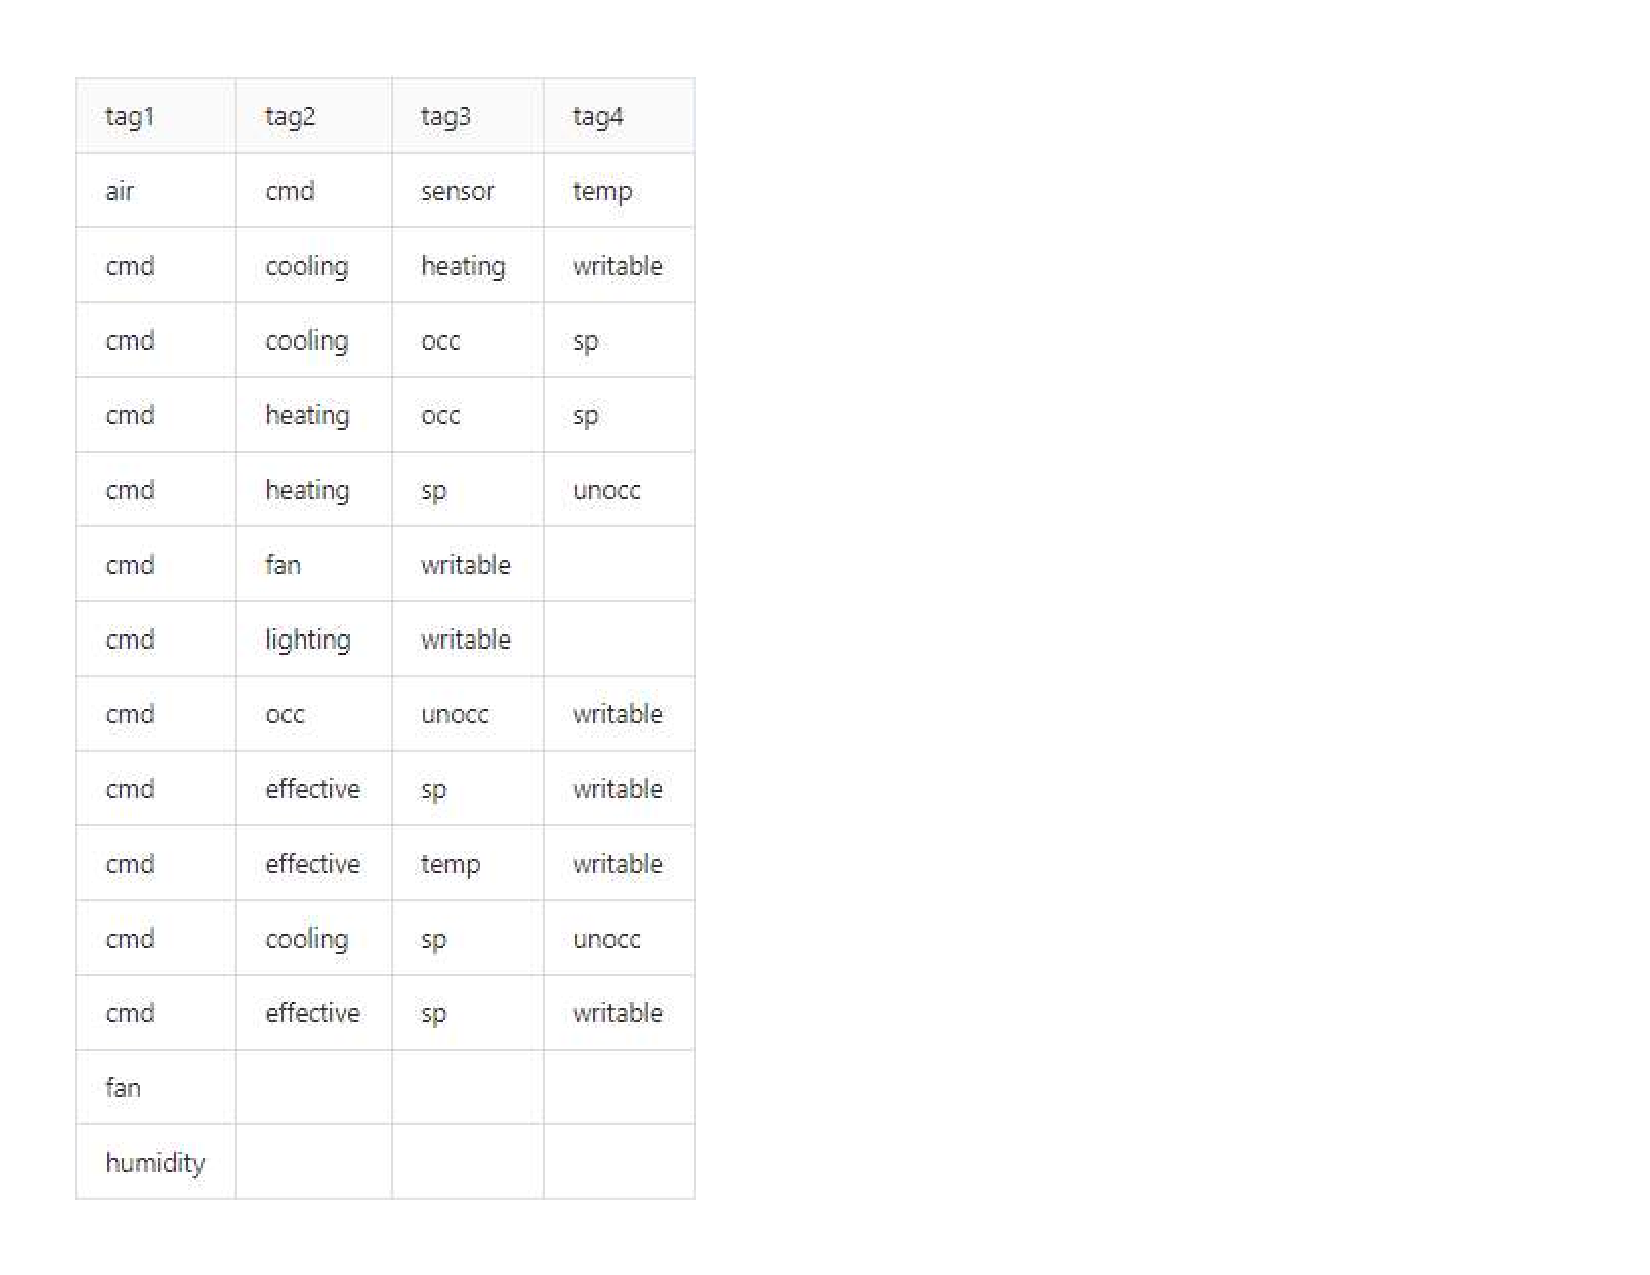
\includegraphics[width=0.30\textwidth,]{tagFilterCoveringArray.pdf}
		\caption{Partial Covering array for tag filtering}
		\label{fig:tagFilterCoveringArray}
	\end{figure}

	With 4 parameters -final tag being default-selected due to a single tag choice being left in the tag dropdown menu- and 13 values each, the amount of tests generated could be vast. 
	However there were three factors that reduced the number of tests to the covering array of Figure~\ref{fig:tagFilterCoveringArray}:
	
	\begin{enumerate}
		\item 13 x 4 lines of constraint logic.
		\item the final tag always being a single choice in the tag-dropdown menu. For example, \textit{humidity} tag has 1 more tag choice available in the dropdown menu, but since it is a single choice it does not affect  the number of tests.
		\item certain points having only so many tags. For example, any point with \textit{fan} or \textit{humidity} having a single tag (+1 tag), and certain combinations of tags - \textit{cmd} \& \textit{fan} or \textit{cmd} \& \textit{lighting} having at most 3 tags (+1 tag).
	\end{enumerate}

	With the test suite of Figure~\ref{fig:tagFilterCoveringArray} generated, only one automation method had to be written and repeated for each test:
	
	\begin{itemize}
		\item the method takes a single argument: a JSON parameter with a predefined string of delimited tags. For example \textit{tagTest1 = "air,cmd,sensor,temp"}; there are 14 similar varieties of tag tests. These are infinitely flexible, simply a different string can be passed in for a different set of tags.
		\item in the method, the string of tags get split by the delimiter. Using these tags, the tag selection is done in an asynchronous for-loop: \emph{for await(tag of tags) \{...\}}. 
		\item as the tags are selected, the panel \& point combinations get filtered. The tag details of the points are verified to match the tags chosen in the filter.
	\end{itemize}
	
	\subsection{Sequenced Filter, Search, Sort of Geo-located Sites}

	The SUT is designed so that the operator can control a number of geo-located sites. 
	The operator has the ability to filter and sort the sites.
	The following functionality is available:
	\begin{itemize}
		\item Sites can be filtered by their status: \textit{Working Well, In Alarm, Disconnected}: 3 Boolean states.
		\item Sites can be filtered by any string entered in the text box.
		\item Sites can be sorted by \textit{Status, Name, Street, Country, Creation Time}
		\item The above actions can happen in any order and should give the same resulting list of filtered and sorted sites.
	\end{itemize}

	The following CTWedge script shows the IPMs for the models of alarm filter and sequence tests. 
	Alarm filters are modeled as 3 Boolean states and the resulting covering array includes 4 configurations. 
	This result is plugged in to the next model, a technique from \cite{ozcan2017applications} to reduce the number of tests and still provide cost effective coverage.
	The parameter \textit{filter-workingWell-inAlarm-disconnected} includes the 4 configurations of these checkboxes as values. 

	\lstset{
    string=[s]{"}{"},
    stringstyle=\color{blue},
    comment=[l]{:},
		commentstyle=\color{black},
		tabsize = 1, %% Sets tab space width.
		showstringspaces = false, %% Prevents space marking in strings, string is defined as the text that is generally printed directly to the console.
		%numbers = left, %% Displays line numbers on the left.
		keywordstyle = \color{blue}, %% Sets  keyword color.
		stringstyle = \color{red}, %% Sets  string color.
		rulecolor = \color{black}, %% Sets frame color to avoid being affected by text color.
		basicstyle = \footnotesize  \ttfamily , %% Sets listing font and size.
		breaklines = true, %% Enables line breaking.
		numberstyle = \tiny,
	}
	\begin{lstlisting}
		Model alarmFilter
	 	Parameters:
			workingWell : Boolean
			InAlarm:  Boolean
			Disconnected : Boolean
		// the result {101, 011, 110, 000} is plugged in to the next model 	
		Model Sequences
		Parameters:
			filter_WW_IA_DC: {101, 011, 110, 000}
			filterBeforeSearch: Boolean
			search : {searchString, siteStreet, siteCity, siteState, siteCountry }
			searchBeforeSort: Boolean
			sortBy:  {status, sName, sStreet, sCountry, createdAt}
			filterBeforeSort: Boolean
	 Constraints: // constraints to reduce address redundancies
	 # filterBeforeSearch=TRUE && searchBeforeSort=TRUE => filterBeforeSort=TRUE #
	 # filterBeforeSearch=FALSE && searchBeforeSort=FALSE => filterBeforeSort=FALSE #
	\end{lstlisting}

	The \textit{search} parameter is a text-box, which is open ended. For this, possible values were contemplated to be any string as well as an assortment of address fields.
	The \textit{sortBy} parameter simply replicates the names of the columns. 
	In order to keep the number of tests low, instead of being a parameter in the model, reverse sorting of columns gets covered in each automated test.
	This is also utilized as a setup \& cleanup in tests since sort order of the previous column gets retained.
	In order to have a deterministic test oracle, an array of sites was generated with varying data parameters - all stored in JSON - so that after filtering by site status and a search string, there would be at least 2 sites to test sorting with.
	
	\begin{figure}[!t]
		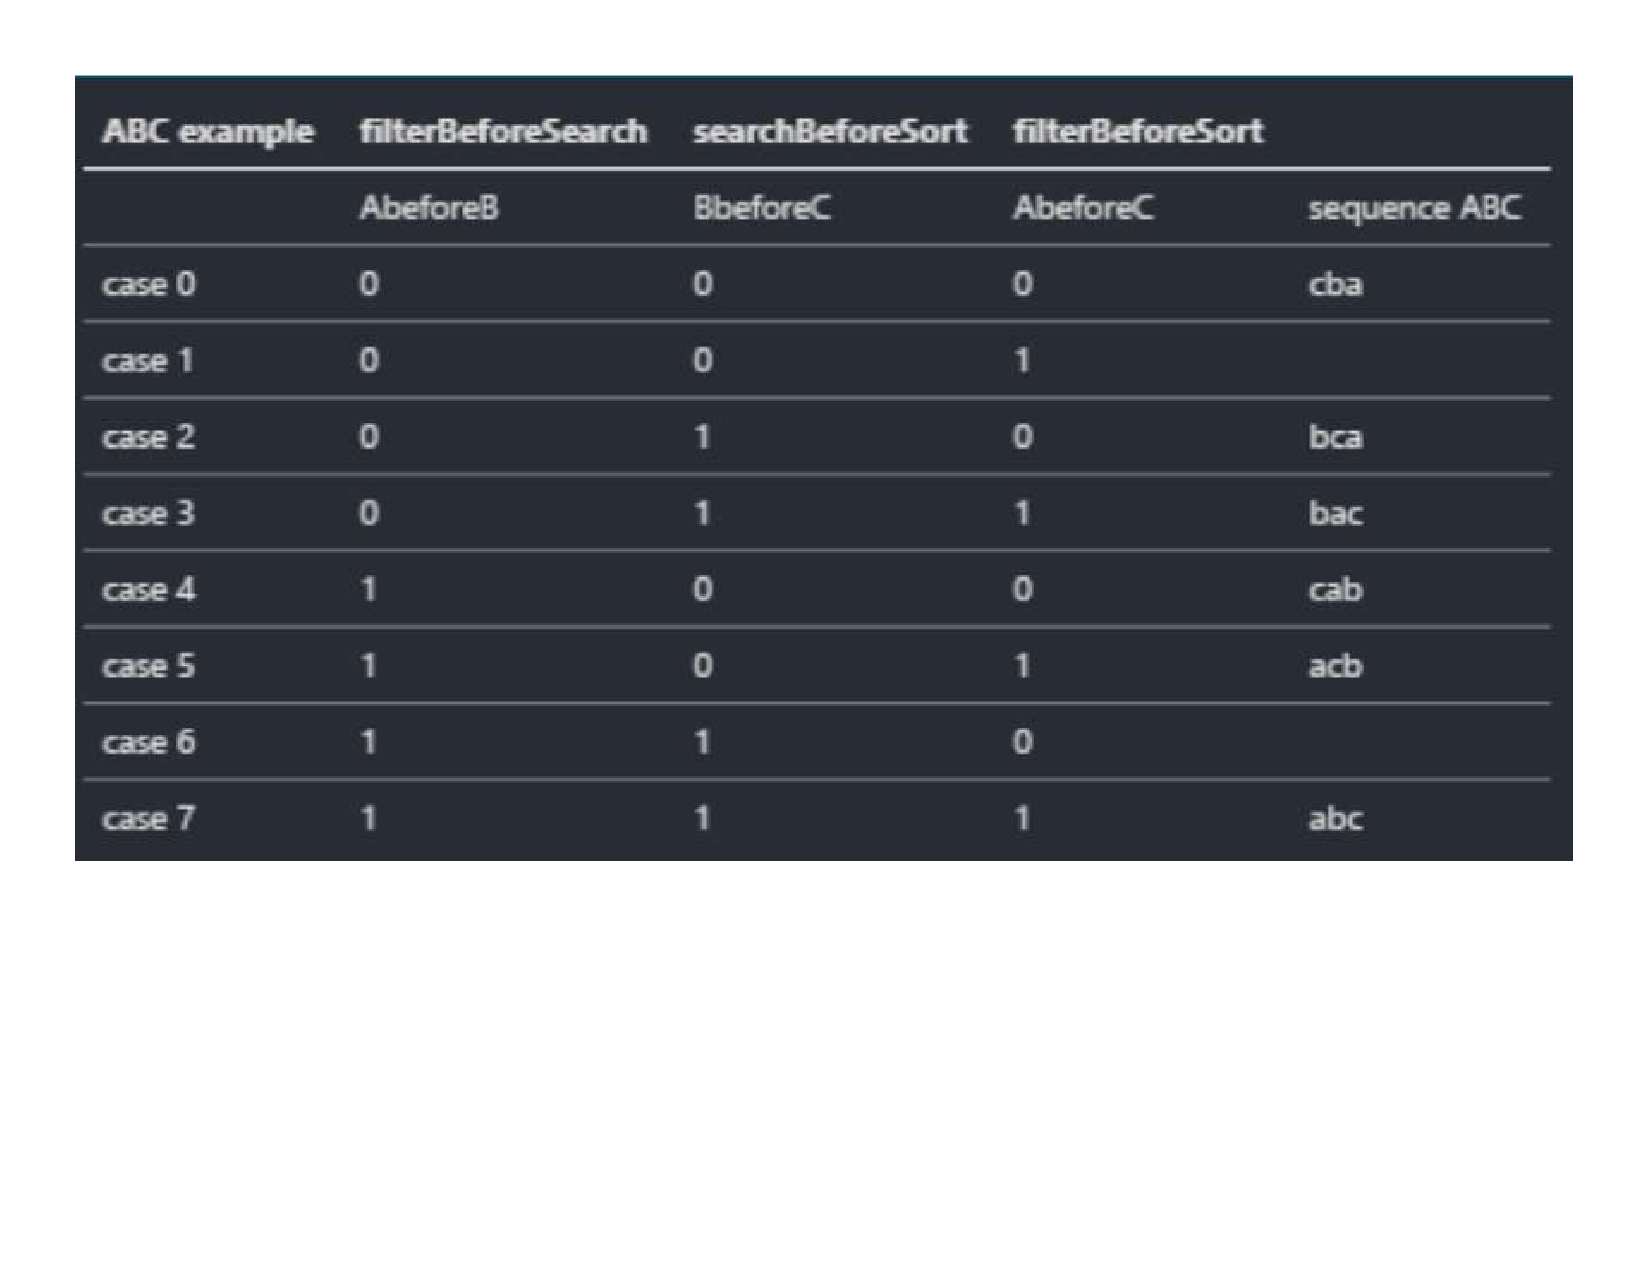
\includegraphics[width=0.50\textwidth,]{sorting.pdf}
		\caption{Sequences of test actions}
		\label{fig:sorting}
	\end{figure}
		
	Finally, the sequence of the user actions needed to be addressed. 
	The two filtering operations and the sorting can happen in any order, and there are 6 possible ways of ordering them.
	If the sequences of the 3 actions \textit{filter, search, sort} were represented as 3 parameters \textit{filterBeforeSearch, searchBeforeSort, filterBeforeSearch}, they could be simplified as \textit{AbeforeB, BbeforeC, AbeforeC}.
	Figure~\ref{fig:sorting} displays this logic in a table.
	As observed, case 1 and case 6 are impossible; if \textit{AbeforeB} and \textit{BbeforeC} have the same Boolean value, \textit{AbeforeC} has to match that value.
	This logic of sequence was addressed with 2 constaints:

	\begin{itemize}
	\item \textit{if filterBeforeSearch is TRUE \&\& searchBeforeSort is TRUE then filterBeforeSort is FALSE}
	\item \textit{if filterBeforeSearch is FALSE \&\& searchBeforeSort is FALSE then filterBeforeSort is TRUE}
	\end{itemize}

	CAMetrics was used to measure pairwise coverage gain per test. 
	The constraints eliminated 5 redundant test cases and the end result became a test suite of 19 tests. With this, a 20.8\% cost saving was achieved while developing automation test code.
	Introducing the Boolean parameters for sequencing and the constraints did not impact the number of test cases; the final number was still 19.

	At a small scale the CT technique used was effective; for 3 parameters, the 6 sequences were possible to be incorporated into the IPM without increasing the number of tests. 
	Also the cost of creating the constraint logic was low since only two constraints had to be written.
	However, it can be observed that with a higher number of parameters this approach can get less cost effective. 
	The team has not encountered such a problem yet and is looking forward to the challenge in a future study.
	
	To conclude this section, the code snippet displays automated Protractor test code for one of the 19 tests.
	The test actions are in the sequence: \textit{search} (by text string), \textit{set site status} (dropdown) and \textit{sort} (by country). 
	The 3 functions execute these actions.
	After so, status pills are verified which verify the site status (In-Alarm, Disconnected, Normal).
	Following that, the sorting and reverse sorting of the sites are verified.
	Finally, the test oracle is verified to check the sites that are displayed as a result of the filters.

	\lstset{
    string=[s]{"}{"},
    stringstyle=\color{blue},
    comment=[l]{:},
		commentstyle=\color{black},
		tabsize = 1, %% Sets tab space width.
		showstringspaces = false, %% Prevents space marking in strings, string is defined as the text that is generally printed directly to the console.
		%numbers = left, %% Displays line numbers on the left.
		keywordstyle = \color{blue}, %% Sets  keyword color.
		stringstyle = \color{red}, %% Sets  string color.
		rulecolor = \color{black}, %% Sets frame color to avoid being affected by text color.
		basicstyle = \footnotesize  \ttfamily , %% Sets listing font and size.
		breaklines = true, %% Enables line breaking.
		numberstyle = \tiny,
	}
	\begin{lstlisting}
    it('should setFilter_110, searchBy_siteCity, sortBy_siteStreet', () => {
      filterAndSort.setFilter(1, 1, 0);
      filterAndSort.textfilter(siteCity);
      filterAndSort.sortSitesBy('Street');
      // alarm pill assertions
      expect(statusWorkingWell).toBeTruthy();
      expect(statusInAlarm).toBeTruthy(); 
      // sorting assertions
      filterAndSort.verifyOrder(expectedOrder);
      // alarm state assertions
      expect(siteInfo.isPresent()).toBeTruthy();
      // reset sorting and clear filters
      filterAndSort.sortSitesBy('Street');
      filterAndSort.xFilters(2);
    });
	\end{lstlisting}


\section{Results, Conclusion and future work}
The tests are executed in CI pipeline environment with every code commit; if the test suite passes, the commit gets checked in and if there is a single failure it does not.
Throughout the effort, defects preventing such check-ins have not been tracked rather fixed on the development branch causing the failure.
On an average, 27\% of the commits run a successful CI pipeline and get merged to the master development branch.
At the time of writing, 157 defects have been found outside of CI pipeline executions and 32 have been found while implementing the automated tests.
There are under 5 thousand lines of automation in Protractor (using TypeScript), more than 300 tests, executing under 600 seconds.
The CI pipeline runs many times a day, at the time of writing there has been 6987 CI pipeline executions in the project.
The tests were written in a 6 month period, by a single developer in test. 
This time included CT modeling, interpreting the model in Protractor code, and all related development and CI activities.

Interpreting the CT model into code is a costly process.To minimize cost in coding time, 2-way strength was utilized and the results achieved in defect prevention were satisfactory for the team. 

In this paper, a variety of CT designs driving e2e UI testing in the front-end of a cloud application have been detailed.
CT was utilized to drive test designs ensuring not only requirement but also high fault-coverage for the functionality under test.
CT assured that the test design process led to writing meaningful and cost-effective automated tests that are more likely to find defects, bolstering confidence in the build quality of the SUT.
All development and test code were unified in the CI pipeline, where every code change results in a full exection of the automated test suite.
Having automated, near-instant feedback with full regression, hundreds of tests running in minutes with each modular code change accellerated development daily.

Consequent of the space restrictions, this study focused on the front-end of the SUT. In the future we plan to study the applications of CT in lower test layers and the CI environment. 

\bibliographystyle{IEEEtran}
\bibliography{cloud}

\end{document}
